\frame{
\frametitle{Bipolaaritransistori}
\begin{itemize}
\item Transistoreja on useita eri tyyppisiä: bipolaaritransistori, MOSFET-transistori,
JFET-transistori, IGBT-transistori \ldots
\item Bipolaaritransistoreja on kahta päätyyppiä: NPN-transistori ja PNP-transistori.
\item MOSFET-transistorit ovat tärkeitä komponentteja, niitä käytetään kytkiminä
sekä mm. tietokoneen prosessoreissa.
\end{itemize}
}


\frame{
\frametitle{NPN-transistori}
\begin{itemize}
\item Perustoiminta: pieni kantavirta ohjaa suurta kollektorivirtaa: $i_{\rm C}=\beta i_{\rm B}$.
\item Kerrointa $\beta$ kutsutaan virtavahvistuskertoimeksi.
\item Kantavirta kulkee vain, jos {\bf kanta-emitteridiodi} johtaa. Kanta-emitteridiodin johtaminen selvitetään kuten tavallisen diodin johtaminen (kynnysjännite: 0,7 volttia).
\item Esimerkiksi, jos kannan ja emitterin välille on kytketty vain 0,4 voltin (joka on alle 0,7 volttia) jännite, diodi ei johda.

\end{itemize}

\begin{center}
\begin{picture}(100,50)(0,-10)
\npn{0,0}{}
\ri{10,0}{I_{\rm B}}
\vln{50,25}{10}
\vln{50,-35}{10}
\di{50,25}{I_{\rm C}}
\di{50,-35}{I_{\rm E}}

\end{picture}
\end{center}

}

\frame{
\frametitle{PNP-transistori}
\begin{itemize}
\item Kuten NPN-transistori, mutta virtojen suunnat ja kanta-emitteridiodin
suunta ovat päinvastaiset!

\end{itemize}

\begin{center}
\begin{picture}(100,50)(0,-10)
\pnp{0,0}{}
\li{0,0}{I_{\rm B}}
\vln{50,25}{10}
\vln{50,-35}{10}
\ui{50,33}{I_{\rm C}}
\ui{50,-24}{I_{\rm E}}

\end{picture}
\end{center}

}

\frame{
\frametitle{Saturaatiotila}
\begin{itemize}
\item Hieman yksinkertaistettuna transistori voidaan ajatella säätimeksi, joka säätelee
kollektorin ja emitterin välistä resistanssia niin, että $i_{\rm C}=\beta i_{\rm B}$.
\item Transistori ei kuitenkaan voi kumota fysiikan lakeja: jos kollektorille on kytketty piiri,
jonka läpi kollektorille voi tulla vain $10 \mA$, niin transistori ei pysty pakottamaan
kollektorivirtaa suuremmaksi kuin tuo $10 \mA$ --- ei, vaikka kannalle syötettäisiin $100 \mA$.
\item Transistorin kollektorin ja emitterin jännitteellä on tietty alaraja, johon se voi laskea.
Tätä alarajaa kutsutaan saturaatiojännitteeksi $U_{\rm CEsat}$.
\item Saturaatiojännite riippuu transistorityypistä: suuruusluokka on tyypillisesti kymmenistä
millivolteista muutamaan sataan millivolttiin.
\end{itemize}
}


\frame{
\frametitle{Laskutekniikkaa}
\begin{itemize}
\item Selvitä ensin, kuinka suuri voi kollektorivirta olla. Eli laske, kuinka suuri olisi kollektorivirta, jos transistori olisi saturaatiotilassa ja $U_{\rm CE}=U_{\rm CEsat}$.
\item Sitten selvitetään kantavirta ja sen perusteella kollektorivirta $i_{\rm C}=\beta i_{\rm B}$.
\item Jos kaavasta $i_{\rm C}=\beta i_{\rm B}$ saatu kollektorivirta on suurempi kuin saturaatiotilalle laskettu
kollektorivirta, transistori on saturaatiossa ja $i_{\rm C}<\beta i_{\rm B}$.
\item Jos kaavasta $i_{\rm C}=\beta i_{\rm B}$ saatu kollektorivirta on pienempi kuin saturaatiotilalle laskettu
kollektorivirta, transistori on aktiivitilassa ja $i_{\rm C}=\beta i_{\rm B}$.
\end{itemize}
Toinen tapa on laskea ensin kantavirta, siitä kollektorivirta ja siitä $U_{\rm CE}$. Jos kollektorin ja emitterin väliseksi jännitteeksi saadaan pienempi jännite kuin transistorin saturaatiojännite, tiedetään, että transistori on saturaatiossa ja kollektorin ja emitterin
välinen jännite on $U_{\rm CEsat}$.
}


\frame{
\frametitle{Esimerkki}
\begin{center}
\begin{picture}(180,100)(0,0)

\vst{0,0}{E_1=5\V}
\vst{200,0}{E_2=12\V}
\vln{200,50}{75}
\vz{100,75}{R_{\rm C}}
\hln{100,125}{100}

\hz{0,50}{R_{\rm B}}
%\txt{75,70}{C\ 1\,\mathrm{nF}}
%\hso{0,50}{K}
%\hln{50,50}{50}
\npn{50,50}{}
\hln{0,0}{200}
\vln{100,0}{25}
\di{100,118}{I_{\rm C}}
\end{picture}

\end{center}
Transistorin virtavahvistuskerroin $\beta=100$, $U_{\rm CEsat}=0,2\V$ ja $R_{\rm B}=5\kohm$.\\
a) Jos $R_{\rm C}=100\ohm$, kuinka suuri on virta $I_{\rm C}$?\\
b) Kuinka suuri saa $R_{\rm C}$:n enintään olla, jotta transistori ei joutuisi saturaatiotilaan?

}


\frame{
\frametitle{Esimerkki}
\begin{center}
\begin{picture}(180,100)(0,10)

\vst{0,0}{E_1=5\V}
\vst{200,0}{E_2=12\V}
\vln{200,50}{75}
\vz{100,75}{R_{\rm C}}
\hln{100,125}{100}

\hz{0,50}{R_{\rm B}}
%\txt{75,70}{C\ 1\,\mathrm{nF}}
%\hso{0,50}{K}
%\hln{50,50}{50}
\npn{50,50}{}
\hln{0,0}{200}
\vln{100,0}{25}
\di{100,118}{I_{\rm C}}
\end{picture}

\end{center}
\scriptsize
Transistorin virtavahvistuskerroin $\beta=100$, $U_{\rm CEsat}=0,2\V$ ja $R_{\rm B}=5\kohm$.\\
a) Jos $R_{\rm C}=100\ohm$, kuinka suuri on virta $I_{\rm C}$?\\
b) Kuinka suuri saa $R_{\rm C}$:n enintään olla, jotta transistori ei joutuisi saturaatiotilaan?\\
a) Kantavirta on $I_{\rm B}=\frac{5\V-0,7\V}{5\kohm}=0,86\mA$. $I_{\rm C}=\beta I_{\rm B}=100\cdot 0,86 \mA=86\mA$. Tarkistetaan vielä, että transistori ei ole saturaatiotilassa: $U_{\rm CE}=E_2-I_{\rm C}R_C=3,4\V$ mikä on suurempi kuin $U_{\rm CEsat}=0,2\V$, eli transistori {\bf ei} ole saturaatiotilassa.\\
b) Transistori on saturaatiotilan rajalla, kun äsken laskettu $I_{\rm C}$ aiheuttaa kollektorin
ja emitterin välille tasan $0,2 \V$ jännitteen. Tällöin $R_{\rm C}$:n yli on $12\V-0,2\V=11,8\V$.
$R_{\rm C}$ saadaan Ohmin laista $R_{\rm C}=\frac{11,8\V}{86\mA}\approx 137\ohm$.
}

\frame{
\frametitle{Toinen esimerkki}
\begin{center}
\begin{picture}(180,100)(0,0)

\vz{0,0}{R_2=10\kohm}
\vz{0,50}{R_1=10\kohm}

\vst{200,0}{E=12\V}
\vln{200,50}{75}
\vz{100,75}{R_{\rm C}}
\hln{100,125}{100}

\hln{0,125}{100}
\vln{0,100}{25}
\hln{0,50}{50}
\npn{50,50}{}
\hln{0,0}{200}
\vln{100,0}{25}
\di{100,118}{I_{\rm C}}
\end{picture}

\end{center}
Transistorin virtavahvistuskerroin $\beta=100$ ja $U_{\rm CEsat}=0,2\V$.\\
a) Jos $R_{\rm C}=100\ohm$, kuinka suuri on virta $I_{\rm C}$?\\
b) Kuinka suuri saa $R_{\rm C}$ enintään olla, jotta transistori ei joutuisi saturaatiotilaan?


}


\frame{
\frametitle{Toinen esimerkki}
Ratkaistaan kantavirta muodostamalla kantapiiristä Théveninin lähde:
\[
E_{\rm T}=E\frac{R_2}{R_1+R_2}=6\V \qquad R_{\rm T}=R_1||R_2=5\kohm
\]
\begin{center}
\begin{picture}(180,150)(0,0)

%\vz{0,0}{R_2=10\kohm}
%\vz{0,50}{R_1=10\kohm}
\vst{0,0}{E_{\rm T}}

\vst{200,0}{E=12\V}
\vln{200,50}{75}
\vz{100,75}{R_{\rm C}}
\hln{100,125}{100}

%\hln{0,125}{100}
%\vln{0,100}{25}
\hz{0,50}{R_{\rm T}}
\npn{50,50}{}
\hln{0,0}{200}
\vln{100,0}{25}
\di{100,118}{I_{\rm C}}
\end{picture}

\end{center}

}

\frame{
\frametitle{Toinen esimerkki}
Nyt kantavirta on
\[
I_{\rm B}=\frac{E_{\rm T}-U_{\rm BE}}{R_{\rm T}}=1,06\mA
\]
Ja kollektorivirta on
\[
I_{\rm C}=\beta I_{\rm B}=106\mA
\]
Kollektorivastuksen yli muodostuu nyt $R_{\rm C}\cdot I_{\rm C}=10,6\V$ jännite, joten $U_{\rm CE}=12\V-10,6\V=1,4\V$ eli suurempi kuin $U_{\rm CEsat}$, eli transistori ei ole saturaatiossa ja kollektorivirta todella on $106\mA$.

B-kohdan raja löytyy, kun selvitetään, millä $R_{\rm C}$:n arvolla $U_{\rm CE}=0,2$, kun kollektorivirta on $106\mA$:
\[
R_{\rm Cmax}=\frac{12\V-0,2\V}{106\mA}\approx 111\ohm.
\]

}

 \frame{
 \frametitle{Releen ohjaaminen transistorilla}
 \begin{itemize}
 \item Esimerkiksi mikrokontrollerin lähtövirta ei yleensä riitä releen ohjaamiseen.
\item Mikrokontrollerin antama 1 milliampeerin virta voidaan transistorilla vahvistaa kymmenien tai satojen milliampeerien suuruiseksi.
\item Kantavastus tulee mitoittaa niin, että rele saa tarpeeksi virtaa ja mikrokontrollerin antama virta ei kasva liian suureksi.
 \end{itemize}
 }

% TODO - piirrä esimerkki:
% Ehdimme käsitellä relettä käyttävän trankun (2 ma mikrokontrolleri, 12 v systeemi, rele vaatii 100 ma, beta)
% ja tulos oli muistaakseni että 1.6-2.6 kohm vastus (mikrokontrolleri 3,3 v)
% muista suojadiodi!
% Piirrä kuva puhtaaksi!

 \frame{
 \frametitle{Releen ohjaaminen transistorilla}
\begin{center}
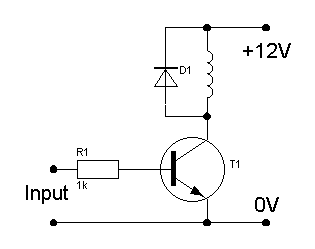
\includegraphics[width=6cm]{transistori_pics/rele.png} % http://www.electro-tech-online.com/electronic-projects-design-ideas-reviews/95934-comparator-not-working-transistor.html
\end{center}

Suojadiodin tarkoitus on mahdollistaa kelan (releen käämin) energian purkautuminen hallitusti, kun transistori katkaisee virran.
 }


 \frame{
 \frametitle{Darlington-kytkentä}
Jos virtavahvistusta tarvitaan paljon, transistorit voidaan kytkeä niin, että ensimmäisen transistorin emitterivirta syötetään toisen transistorin kannalle. Piiriä kutsutaan Darlington-kytkennäksi.
\begin{center}
\begin{picture}(100,100)(0,0)

\npn{0,50}{}
\npn{50,25}{}

\hln{50,75}{50}
\vln{100,50}{50}
%\vln{100,100}{25}

\out{0,50}
\out{100,-25}
\out{100,100}
\vln{100,-25}{25}

\di{100,90}{I_1}
\ri{10,50}{I_2}

\end{picture}

\end{center}
 }

% TODO: Kerro Darlingtonin ja Sziklain eroista ja miksi ko. kytkentöjä käytetään.
% Ks. myös http://www.inner-magazines.com/news/50/66/60-Years-of-Audio-Transistors/

\frame{
\frametitle{Esimerkki: Sziklai-kytkentä}
\begin{center}
\begin{picture}(100,100)(0,0)

\npn{0,50}{}
\pnpc{50,75}{}

\hln{50,25}{50}
\vln{100,0}{50}
\vln{100,100}{25}

\out{0,50}
\out{100,0}
\out{100,125}

\di{100,115}{I_1}
\ri{10,50}{I_2}

\end{picture}

\end{center}
Laske koko piirin virtavahvistus $\beta_{\rm kok}=\frac{I_1}{I_2}$. Molemmilla transistoreilla on sama virtavahvistus $\beta$ (ei lukuarvoa).

}


\frame{
\frametitle{Esimerkki: Sziklai-kytkentä}
\begin{center}
\begin{picture}(100,100)(0,0)

\npn{0,50}{}
\pnpc{50,75}{}

\hln{50,25}{50}
\vln{100,0}{50}
\vln{100,100}{25}

\out{0,50}
\out{100,0}
\out{100,125}

\di{100,115}{I_1=\beta^2I_2+\beta I_2}
\ri{10,50}{I_2}

\li{55,75}{\beta I_2}
\di{100,40}{\beta\beta I_2=\beta^2I_2}

\end{picture}

\end{center}
\[
\beta_{\rm kok}=\frac{I_1}{I_2}=\frac{\beta^2I_2+\beta I_2}{I_2}=\beta^2 + \beta
\]
}

